\renewcommand*{\arraystretch}{1.1}

\subsection*{Interactive / complex / 3}
\label{sec:interactive-complex-read-03}

\noindent\begin{tabularx}{\queryCardWidth}{|>{\queryPropertyCell}c|X|}
	\hline
	query & Interactive / complex / 3 \\ \hline
%
	title & Friends and friends of friends that have been to countries X and Y \\ \hline
%
	pattern & \hfill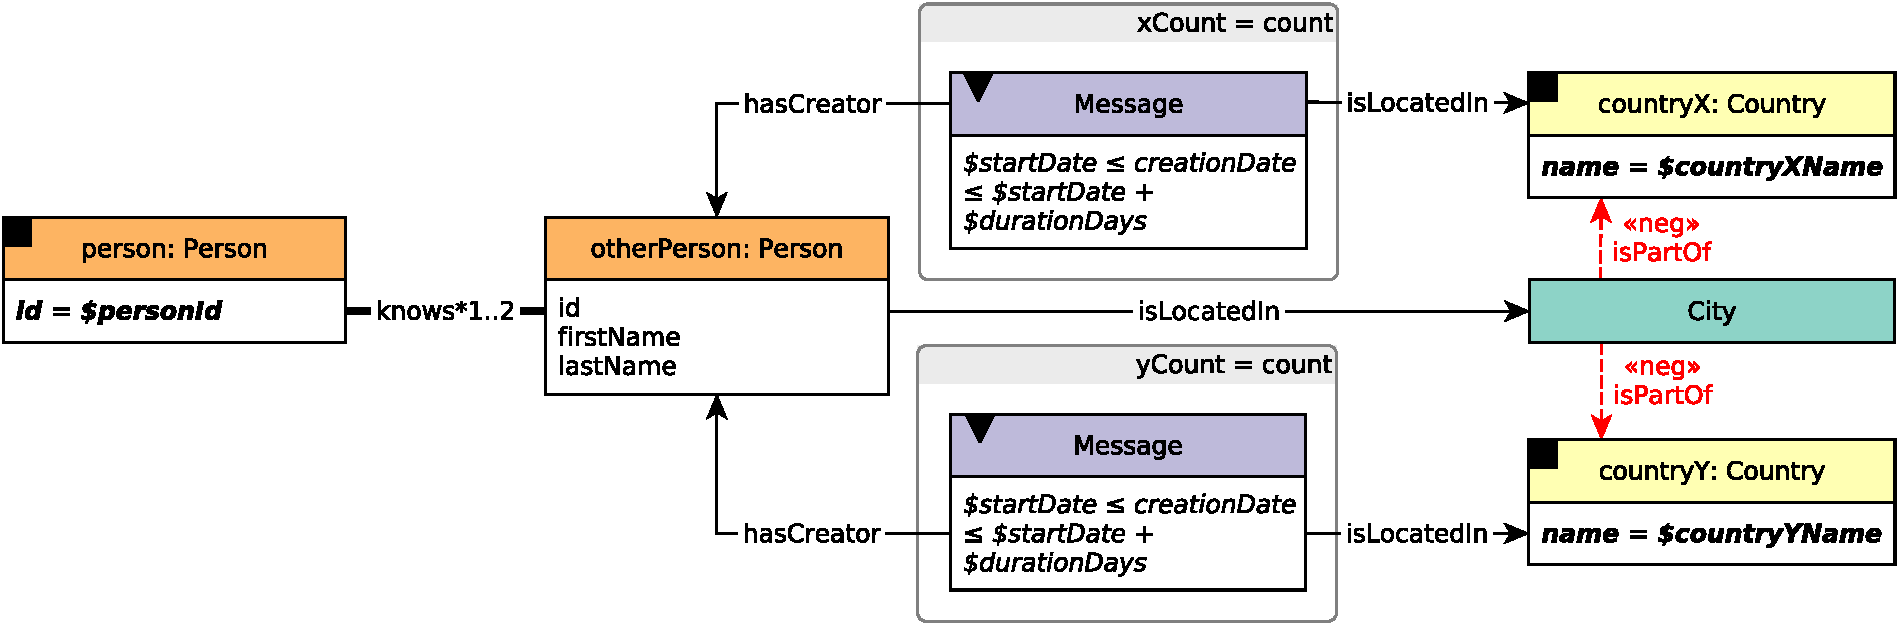
\includegraphics[scale=\patternscale,margin=0cm .2cm]{patterns/interactive-complex-read-03}\hfill\vadjust{} \\ \hline
%
	desc. & Given a start Person, find Persons that are their friends and friends of
friends (excluding start Person) that have made Posts/Comments in both
of the given Countries, X and Y, within a given period. Only Persons
that are foreign to Countries X and Y are considered, that is Persons
whose Location is not Country X or Country Y.
 \\ \hline
%
	
%
	
		params &
		\innerCardVSpace{\begin{tabularx}{\attributeCardWidth}{|>{\paramNumberCell}c|>{\varNameCell}M|>{\typeCell}m{\typeWidth}|Y|} \hline
		$\mathsf{1}$ & Person.id & ID &  \\ \hline
		$\mathsf{2}$ & CountryX.name & String &  \\ \hline
		$\mathsf{3}$ & CountryY.name & String &  \\ \hline
		$\mathsf{4}$ & startDate & Date & beginning of requested period \\ \hline
		$\mathsf{5}$ & duration & 32-bit Integer & duration of requested period, in days the interval [startDate, startDate + Duration) is closed-open \\ \hline
		\end{tabularx}}\innerCardVSpace \\ \hline
	
%
	
		result &
		\innerCardVSpace{\begin{tabularx}{\attributeCardWidth}{|>{\resultNumberCell}c|>{\varNameCell}M|>{\typeCell}m{\typeWidth}|>{\resultOriginCell}c|Y|} \hline
		$\mathsf{1}$ & Person.id & ID &R&
				 \\ \hline
		$\mathsf{2}$ & Person.firstName & String &R&
				 \\ \hline
		$\mathsf{3}$ & Person.lastName & String &R&
				 \\ \hline
		$\mathsf{4}$ & countX & 32-bit Integer &A&
				number of Messages from Country X made by Person within the given time \\ \hline
		$\mathsf{5}$ & countY & 32-bit Integer &A&
				number of Messages from Country Y made by Person within the given time \\ \hline
		$\mathsf{6}$ & count & 32-bit Integer &A&
				countX + countY \\ \hline
		\end{tabularx}}\innerCardVSpace \\ \hline
	
%
	sort		&
		\innerCardVSpace{\begin{tabular}{|>{\sortNumberCell}c|>{\varNameCell}l|>{\directionCell}c|} \hline
		$\mathsf{1}$ & countX & $\desc$ \\ \hline
		$\mathsf{2}$ & Person.id & $\asc$ \\ \hline
		\end{tabular}}\innerCardVSpace \\ \hline
	%
	limit & 20 \\ \hline
	%
	CPs &
	\multicolumn{1}{>{\raggedright}l|}{
		\chokePoint{2.1}, 
		\chokePoint{3.1}, 
		\chokePoint{5.1}
		} \\ \hline
	%
	relevance &
		\small This query looks for paths of length two and three, starting from a Person, going to friends or friends of friends, and
then moving to Messages. This query tests the ability of the query optimizer to select the most efficient join ordering,
which will depend on the cardinalities of the intermediate results. Many friends of friends can be duplicate, then it is
expected to eliminate duplicates and those people prior to access the Post and Comments, as well as eliminate those
friends from countries X and Y, as the size of the intermediate results can be severely affected. A possible structural
optimization could be to materialize the number of Posts and Comments created by a person, and progressively
filter those people that could not even fall in the top 20 even having all their posts in the countries X and Y.
 \\ \hline%
\end{tabularx}
\queryCardVSpace